\section{TOPSIS}

\begin{definition}[TOPSIS]
    TOPSIS 法，全称为“逼近理想解排序法”，是多属性决策分析中一种常用且有效的技术。基于数据，构建出一个虚拟的“最优方案”（即正理想解和一个虚拟的“最劣方案”（即负理想解）。

    然后，通过计算每一个评价对象与这两个虚拟方案的相对接近程度，来进行排序。一个好的方案，应该距离最优方案最近，同时距离最劣方案最远。
\end{definition}

\subsection{指标正向化}

\begin{center}
    \begin{tabular}{|c|c|c|}
        \hline 指标名称       & 指标特点     & 例子            \\
        \hline 极大型（效益型）指标 & 越大（多）越好  & 成绩、GDP增速、企业利润 \\
        \hline 极小型（成本型）指标 & 越小（少）越好  & 费用、坏品率、污染程度   \\
        \hline 中间型指标      & 越接近某个值越好 & 水质量评估时的PH值    \\
        \hline 区间型指标      & 落在某个区间最好 & 体温、水中植物性营养物量  \\
        \hline
    \end{tabular}
\end{center}

\begin{theorem}[指标正向化]
    1．极小型指标
    $$
        \max -x
    $$
    如果所有的元素均为正数，那么也可以使用
    $$
        \frac{1}{x}
    $$
    2．中间型指标：
    $\left\{x_i\right\}$ 是一组中间型指标序列，且最佳的数值为 $x_{b e s t}$ ，那么正向化的公式如下：
    $$
        M=\max \left\{\left|x_i-x_{b e s t}\right|\right\}, \quad \tilde{x}_i=1-\frac{\left|x_i-x_{b e s t}\right|}{M}
    $$
    3．区间型指标：
    $\left\{x_i\right\}$ 是一组区间型指标序列，且最佳的区间为 $[a, b]$ ，那么正向化的公式如下：
    $$
        \begin{aligned}
             & M=\max \left\{a-\min \left\{x_i\right\}, \max \left\{x_i\right\}-b\right\}, \tilde{x}_i= \begin{cases}1-\frac{a-x_i}{M} & , x_i<a             \\
             1                 & , a \leq x_i \leq b \\
             1-\frac{x_i-b}{M} & , x_i>b\end{cases}
        \end{aligned}
    $$
\end{theorem}

\begin{lstlisting}[language=python]
def min2max(datas: list, offset=1e-9) -> list:
    def normalization(data) -> float:
        return 1 / (data + offset)

    return list(map(normalization, datas))


# 最佳范围被认为是中点
def middle2max(datas, x_min, x_max):
    def normalization(data):
        if data <= x_min or data >= x_max:
            return 0
        elif data > x_min and data < (x_min + x_max) / 2:
            return 2 * (data - x_min) / (x_max - x_min)
        elif data < x_max and data >= (x_min + x_max) / 2:
            return 2 * (x_max - data) / (x_max - x_min)

    return list(map(normalization, datas))


def interval2max(datas, x_min, x_max, x_tolerant_min, x_tolerant_max):
    def normalization(data):
        if data >= x_min and data <= x_max:
            return 1
        elif data <= x_tolerant_min or data >= x_tolerant_max:
            return 0
        elif data > x_max and data < x_tolerant_max:
            return 1 - (data - x_max) / (x_tolerant_max - x_max)
        elif data < x_min and data > x_tolerant_min:
            return 1 - (x_min - data) / (x_min - x_tolerant_min)

    return list(map(normalization, datas))
\end{lstlisting}

\subsection{计算过程}

考虑边际效应，在某些正向化数值较大的情况下，
再增加相同数值所带来的感知提升就越小，
可据此将正向标准化的线性假设（Linear Assumption）
转化为对数假设（Logarithmic Hypothesis），
则这两个参数的式子设置为：
\begin{equation}
    R_{ij} = ln(X_{ij} + 1)
\end{equation}

$X_{ij} + 1$ 是为了防止 $X_{ij} = 0$ 时对数函数无意义。

指标正向化后，使用TOPSIS-熵权法来确定这些参数的权重。
我们构建 $m$ 个事物 $n$ 个评价指标的判断矩阵 $R_{ij}(i, j \in \mathbb{Z}^+)$，并将判断矩阵进行归一化处理，得到新的归一化判断矩阵 $B$，矩阵 $B$ 的元素获取公式为：
\begin{equation}
    B_{ij} = \frac{R_{ij} - \min_{1 \le k \le m}\{R_{kj}\}}{\max_{1 \le k \le m}\{R_{kj}\} - \min_{1 \le k \le m}\{R_{kj}\}}
\end{equation}

计算第 $i$ 个对象在第 $j$ 个指标下的值占该指标总值的比例 $p_{ij}$：
\begin{equation}
    p_{ij} = \frac{x_{ij}}{\sum_{k=1}^{m} x_{kj}}
\end{equation}

这样得到了比例矩阵 $\mathbf{P} = (p_{ij})_{m \times n}$。而第 $j$ 个指标的信息熵 $e_j$ 计算公式如下：
\begin{equation}
    e_j = -k \sum_{i=1}^{m} (p_{ij} \ln(p_{ij}))
\end{equation}

$k = \frac{1}{\ln(m)}$ 为调节系数，注意在 $m = 1$时需要特殊处理（如返回均等权重）。

接下来，将各指标的差异度进行归一化，得到最终的熵权 $w_j$：
\begin{equation}
    w_j = \frac{1 - e_j}{\sum_{i=1}^{n} (1 - e_i)}
\end{equation}

熵权得到后，我们采用 TOPSIS - 熵权法计算综合得分，首要步骤为确定最优解向量 $Z^+$ 和最劣解向量 $Z^-$。$Z^+$ 是归一化判断矩阵 $B$ 中每列的最大值组成的向量；$Z^-$ 是归一化判断矩阵 $B$ 中每列的最小值组成的向量。其计算公式分别为：
\begin{equation}
    Z^+ = \left(\max_{1 \leq i \leq m}\{B_{i1}\}, \max_{1 \leq i \leq m}\{B_{i2}\}, \cdots, \max_{1 \leq i \leq m}\{B_{in}\}\right)
\end{equation}

\begin{equation}
    Z^- = \left(\min_{1 \leq i \leq m}\{B_{i1}\}, \min_{1 \leq i \leq m}\{B_{i2}\}, \cdots, \min_{1 \leq i \leq m}\{B_{in}\}\right)
\end{equation}

在熵权法中，使用的权重 $w_j$ 进行加权处理。
第 $i$ 个方案到最优解向量 $Z^+$ 的距离 $D_i^+$ 和到最劣解向量 $Z^-$ 的距离 $D_i^-$ 的公式分别为：
\begin{equation}
    D_i^+ = \sqrt{\sum_{j = 1}^{n} w_j (B_{ij} - Z_j^+)^2}, \quad 	D_i^- = \sqrt{\sum_{j = 1}^{n} w_j (B_{ij} - Z_j^-)^2}
\end{equation}

最终只需相对接近度 $C_i$（第 $i$ 个方案与最优解的相对接近程度），即可视为综合得分，其计算公式为：
\begin{equation}
    C_i = \frac{D_i^-}{D_i^+ + D_i^-}
\end{equation}

这些流程的代码如下所示：

\begin{lstlisting}[language=python]
def batch_normalize_from_rules(df, rules: list) -> pd.DataFrame:
    """读取规则列表，批量处理数据 DataFrame"""
    for rule in rules:
        column_name = rule['column']
        datas = df[column_name].tolist()

        type_to_func = {'max': max2max, 'min': min2max, 'middle': middle2max, 'interval': interval2max}
        func_to_call = type_to_func.get(rule['type'])

        normalized_values = func_to_call(datas, **rule['params'])
        df[column_name] = normalized_values

    return df


def normalization(df: pd.DataFrame) -> pd.DataFrame:
    return df / np.sqrt((df ** 2).sum())


def entropyWeight(df):
    """计算第 j 个指标下第 i 个样本所占的比重"""
    df = np.array(df)
    P = df / df.sum(axis=0)
    E = np.nansum(-P * np.log(P) / np.log(len(df)), axis=0)
    d = (1 - E)
    W = d / d.sum()
    return W


def topsis(data, weight):
    # 最优最劣方案（Z+ 和 Z-）
    Z = pd.DataFrame([data.max(), data.min()], index=['Z+', 'Z-'])
    weight = entropyWeight(data) if weight is None else np.array(weight)
    result = data.copy()
    result['Z+'] = np.sqrt(((data - Z.loc['Z+']) ** 2 * weight).sum(axis=1))  # 评价对象与最大值的距离
    result['Z-'] = np.sqrt(((data - Z.loc['Z-']) ** 2 * weight).sum(axis=1))
    result['综合得分指数'] = result['Z-'] / (result['Z-'] + result['Z+'])
    result['排序'] = result.rank(ascending=False)['综合得分指数']

    return result, Z, weight
\end{lstlisting}

\begin{tips}
    TOPSIS 的数据呈现可以用绘图，使用雷达图来呈现。

    \href{https://matplotlib.org/stable/gallery/specialty_plots/radar_chart.html}{https://matplotlib.org/stable/gallery/specialty\_plots/radar\_chart.html}
\end{tips}

\begin{figure} [H]
    \centering
    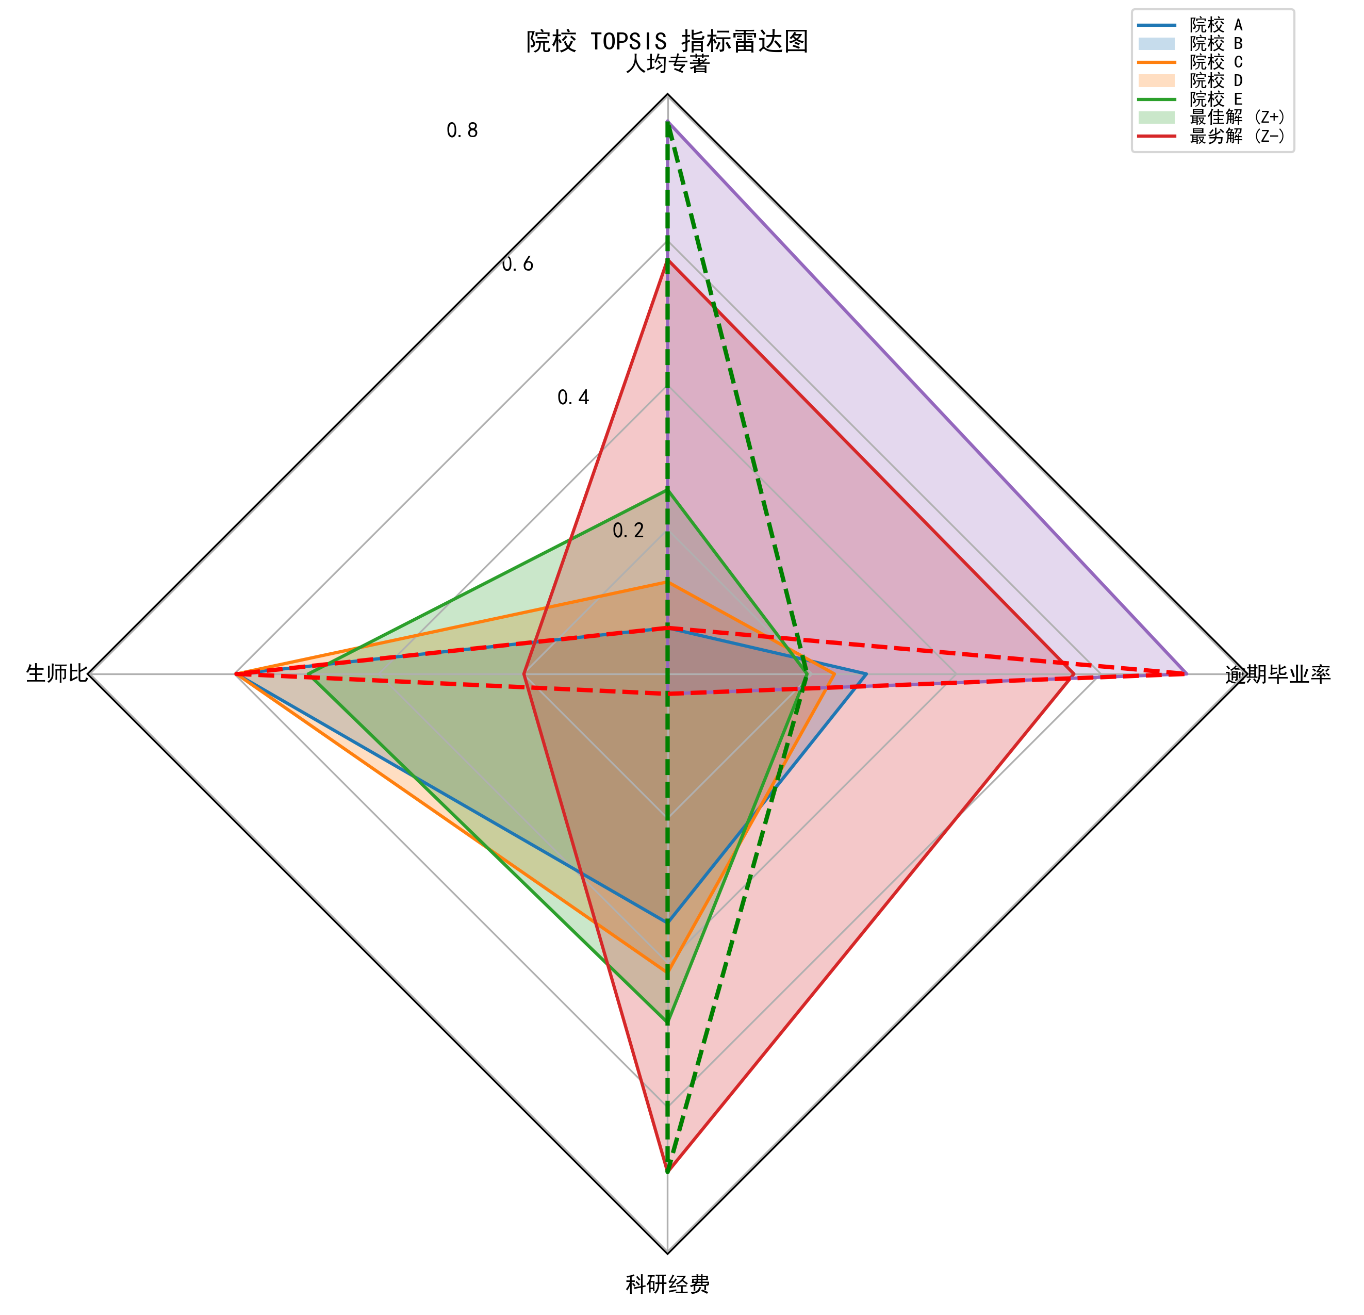
\includegraphics[width=0.5\textwidth]{chapters/评价类模型/images/TOPSIS/img-20250821215353.png}
\end{figure}

\subsection{优点}

\begin{itemize}
    \item 原理直观: 几何意义清晰，易于理解。
    \item 计算简便: 算法流程清晰，易于编程实现。
    \item 适用性广: 对样本量和指标数量没有严格限制，对数据分布也无特殊要求。
    \item 结果合理: 能够充分利用原始数据信息，得出的排序结果较为合理。
\end{itemize}

\subsection{缺点}

\begin{itemize}
    \item 权重依赖性: 指标权重的确定带有一定的主观性，不同的权重设置可能导致不同的结果。
    \item 排序的相对性: 当新增或删除方案时，可能会导致各方案的排序发生变化（秩逆转）。
    \item 规范化方法影响: 不同的数据规范化方法可能会对最终结果产生影响。
\end{itemize}